\documentclass[10pt]{beamer}

% === Theme ===
\usetheme{metropolis}
\setbeamertemplate{frame footer}{\insertshortauthor\quad|\quad\insertshortinstitute}

% === Packages ===
\usepackage[T1]{fontenc}
\usepackage{graphicx}
\usepackage{booktabs}
\usepackage{amsmath,amssymb}
\usepackage{listings}
\usepackage{xcolor}
\usepackage{tikz}
\usepackage{array}

% === lstlisting style for compiled rules ===
\lstset{
  basicstyle=\scriptsize\ttfamily,
  breaklines=true,
  frame=single,
  numbers=none,
  aboveskip=4pt,
  belowskip=4pt,
  backgroundcolor=\color{gray!5},
  columns=fullflexible,
  keepspaces=true,
  xleftmargin=4pt,
  xrightmargin=4pt,
}

% === Tighten spacing ===
\setbeamertemplate{itemize item}{\textbullet}
\setbeamertemplate{itemize subitem}{--}

% === Metadata ===
\title{Interpretable Card-Play Strategies\\from Evolved Logic Networks}
\subtitle{A Neurosymbolic Agent for Sueca}
\author[A. Cardoso]{André Cardoso}
\institute[U. Aveiro]{DETI, Universidade de Aveiro}
\date{June 2026}

\begin{document}

% ======================================================================
% SLIDE 1 — Title
% ======================================================================
\begin{frame}[plain]
  \maketitle
\end{frame}

% ======================================================================
% SLIDE 2 — Problem & Motivation
% ======================================================================
\begin{frame}{Most strong card-playing AIs are black boxes: can competitive play be human-auditable?}
  \begin{columns}[T]
    \column{0.48\textwidth}
      \begin{block}{The status quo}
        \footnotesize
        Deep PIMC and neural policy nets.\\[6pt]
        Millions of floating-point weights $\rightarrow$ \textbf{opaque}.\\[6pt]
        \textit{``Why did you play that card?''}\\
        \textit{``\ldots the matrix says so.''}
      \end{block}
    \column{0.48\textwidth}
      \begin{block}{Our goal}
        \footnotesize
        Evolved logic gates.\\[6pt]
        A handful of \textbf{human-readable IF/THEN rules}.\\[6pt]
        \textit{``I duck because the trick is cheap and I want to build a void.''}
      \end{block}
  \end{columns}
  \vspace{10pt}
  \centering
  \textbf{Thesis:} discrete logic gates $+$ neuroevolution $\rightarrow$ competitive play \textit{and} interpretability.
\end{frame}

% ======================================================================
% SLIDE 3 — Sueca in 60 seconds
% ======================================================================
\begin{frame}{Sueca's distinctive rules create a rich strategic texture}
  \begin{columns}[T]
    \column{0.50\textwidth}
      \textbf{Table layout} {\footnotesize\textit{(4 players, 2 teams)}}\\[4pt]
      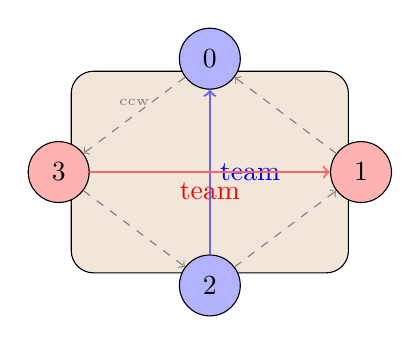
\begin{tikzpicture}[scale=0.80]
        % Table
        \draw[rounded corners=8pt,fill=brown!20] (-2.2,-1.6) rectangle (2.2,1.6);
        % Seats
        \node[circle,draw,fill=blue!30,inner sep=0pt,minimum size=22pt] (S0) at (0,1.8) {0};
        \node[circle,draw,fill=red!30,inner sep=0pt,minimum size=22pt] (S3) at (-2.4,0) {3};
        \node[circle,draw,fill=blue!30,inner sep=0pt,minimum size=22pt] (S2) at (0,-1.8) {2};
        \node[circle,draw,fill=red!30,inner sep=0pt,minimum size=22pt] (S1) at (2.4,0) {1};
        \draw[<-,thick,blue!60] (S0) -- (S2) node[midway,right,blue] {team};
        \draw[<-,thick,red!60] (S1) -- (S3) node[midway,below,red] {team};
        % Turn order
        \draw[->,dashed,gray] (S0) -- (S3) node[midway,above,font=\tiny] {ccw};
        \draw[->,dashed,gray] (S3) -- (S2);
        \draw[->,dashed,gray] (S2) -- (S1);
        \draw[->,dashed,gray] (S1) -- (S0);
      \end{tikzpicture}
    \column{0.50\textwidth}
      \textbf{Key rules}\\[4pt]
      \begin{itemize}
        \item \textbf{40 cards} (no 8,9,10)
        \item Rank: \textbf{A > 7 > K > J > Q > 6--2}
        \item 7 = \textit{manilha} (2nd-highest!)
        \item \textbf{120 points/deal}; game-point tiers
        \item Must \textbf{follow suit}; trump cuts
        \item \textbf{Public void tracking}
        \item Imperfect information:\\
              you see only your hand + history
      \end{itemize}
  \end{columns}
  \vspace{4pt}
  \centering
  \small\emph{These rules define the strategic vocabulary the WANN must learn.}
\end{frame}

% ======================================================================
% SLIDE 4 — Architecture (arch.pdf)
% ======================================================================
\begin{frame}{The agent reads a public-information belief state through evolved logic gates and outputs a strategic intent}
  \centering
  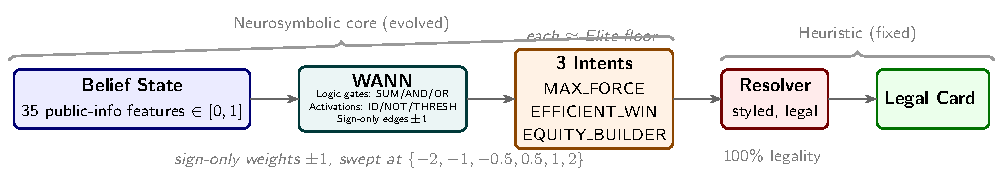
\includegraphics[width=\textwidth,height=0.55\textheight,keepaspectratio]{../report/figures/arch.pdf}
  \vspace{4pt}
  \begin{columns}[T]
    \column{0.33\textwidth}
      \centering\scriptsize
      \textbf{35 belief features}\\
      Hand, trick state, voids,\\
      boss detection, ``can I win?''
    \column{0.33\textwidth}
      \centering\scriptsize
      \textbf{3 intents}\\
      MAX\_FORCE, EFFICIENT\_WIN,\\
      EQUITY\_BUILDER
    \column{0.33\textwidth}
      \centering\scriptsize
      \textbf{Styled resolver}\\
      Every intent $\approx$ Elite;\\
      100\% legal outputs
  \end{columns}
\end{frame}

% ======================================================================
% SLIDE 5 — WANN concept
% ======================================================================
\begin{frame}{Weight-agnostic networks replace learned weights with evolved logic-gate topology}
  \begin{columns}[T]
    \column{0.52\textwidth}
      \textbf{Node types}\\[4pt]
      {\footnotesize
      \begin{tabular}{@{}ll@{}}
        \toprule
        \textbf{Aggregation} & \textbf{Activation} \\
        \midrule
        SUM $\Sigma x_i$ & IDENTITY $x$ \\
        MIN $=$ AND      & NOT $1{-}x$ \\
        MAX $=$ OR       & THRESHOLD $x{>}0.5$ \\
        \bottomrule
      \end{tabular}}
      \vspace{8pt}
      \begin{itemize}
        \item No MEAN (precision), no SIGMOID (rules)
        \item All outputs clamped to $[0,1]$
      \end{itemize}
    \column{0.48\textwidth}
      \textbf{Why it compiles to rules}\\[4pt]
      \begin{itemize}
        \item Connections: \textbf{sign only} ($\pm 1$)
        \item Shared weight sweep:\\[-2pt]
              $W \in \{-2,-1,-0.5,\,0.5,1,2\}$
        \item Topology must work at \emph{all} scales
        \item Every gate is a logic primitive\\
              $\rightarrow$ \textbf{Boolean-ish rules}
        \item Tie-breaking: \textbf{random} among max intents
      \end{itemize}
  \end{columns}
  \vspace{6pt}
  \centering
  \small\emph{The architecture constraint \textbf{is} the interpretability guarantee.}
\end{frame}

% ======================================================================
% SLIDE 6 — Training Pipeline
% ======================================================================
\begin{frame}{Training bootstraps on expert demonstrations then switches to co-evolutionary self-play}
  \centering
  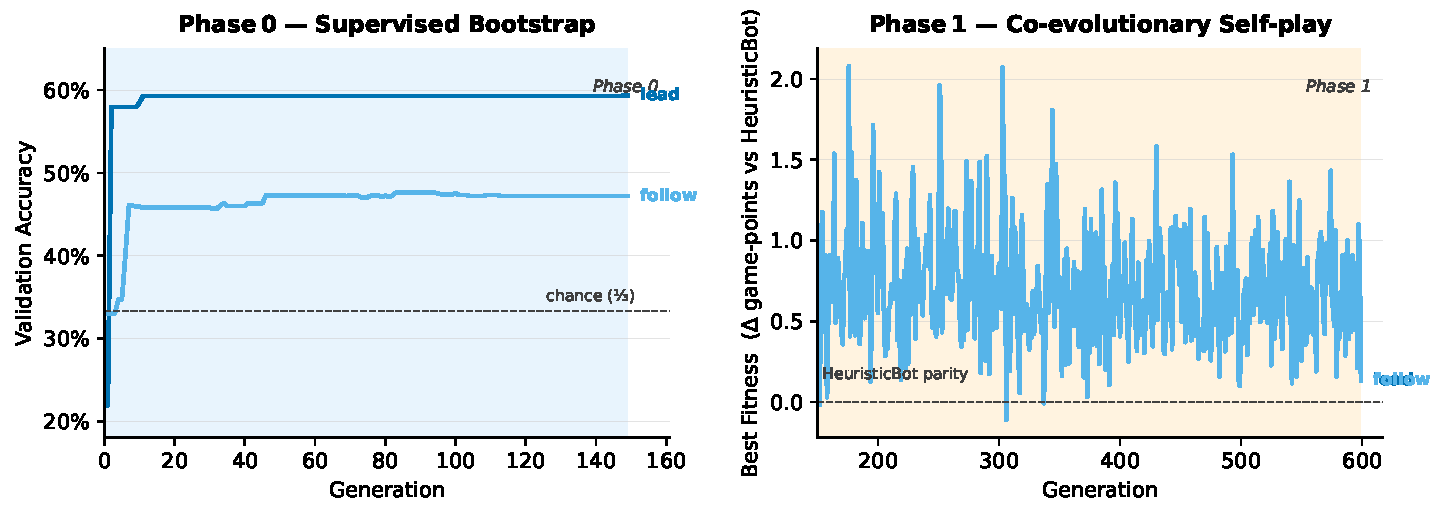
\includegraphics[width=0.78\textwidth,height=0.42\textheight,keepaspectratio]{../report/figures/training_curve.pdf}
  \vspace{4pt}
  \begin{columns}[T]
    \column{0.50\textwidth}
      \centering
      \textbf{Phase 0 (gens 0--149)}\\
      \scriptsize
      Supervised pretraining on PIMC data\\
      PFS-NEAT from \textbf{zero} connections\\
      Split: \textit{lead} vs.\ \textit{follow} datasets\\
      Adaptive 2-stage mutation filter
    \column{0.50\textwidth}
      \centering
      \textbf{Phase 1 (gens 150--599)}\\
      \scriptsize
      Co-evolutionary self-play\\
      Dynamic per-decision brain routing\\
      Delta-fitness with CRN\\
      HOF + MAP-Elites opponent pools
  \end{columns}
\end{frame}

% ======================================================================
% SLIDE 7 — The Rollout Teacher
% ======================================================================
\begin{frame}{A cheap supra-Elite teacher made the champion 4.5$\times$ simpler at equal strength}
  \begin{columns}[T]
    \column{0.48\textwidth}
      \footnotesize
      \textbf{Problem diagnosed}\\[2pt]
      \begin{itemize}
        \item Deep PIMC \textbf{only tied} Elite
        \item Root cause: \textbf{myopic leaf eval} (raw score, no positional estimate)
        \item Depth doesn't fix a blind leaf
      \end{itemize}
      \vspace{4pt}
      \textbf{Solution}\\[2pt]
      \begin{itemize}
        \item Flat Monte-Carlo PIMC + \textbf{Elite playouts}
        \item Rollout policy improvement: $\text{1-ply} + \text{Elite} \ge \text{Elite}$
        \item \textbf{62\% vs.\ Elite}, $\sim$1000$\times$ faster
      \end{itemize}
    \column{0.52\textwidth}
      \centering
      \textbf{What the better teacher bought}\\[4pt]
      \begin{tabular}{@{}lcc@{}}
        \toprule
        & \textbf{Earlier} & \textbf{Final} \\
        \midrule
        vs.\ Elite     & 52.7\%           & \textbf{52.1\%} \\
        Hidden gates   & 132              & \textbf{29} \\
        Connections    & 188              & \textbf{49} \\
        Teacher        & $\alpha$-$\beta$ & \textbf{rollout} \\
        \bottomrule
      \end{tabular}
      \vspace{8pt}
      \centering
      \small\emph{Stronger teacher $\rightarrow$ simpler champion.\\The ceiling is the resolver, not the teacher.}
  \end{columns}
\end{frame}

% ======================================================================
% SLIDE 8 — Results
% ======================================================================
\begin{frame}{The champion beats Elite 52.1\% $\pm$ 1.8\% ($n=3000$)}
  \centering
  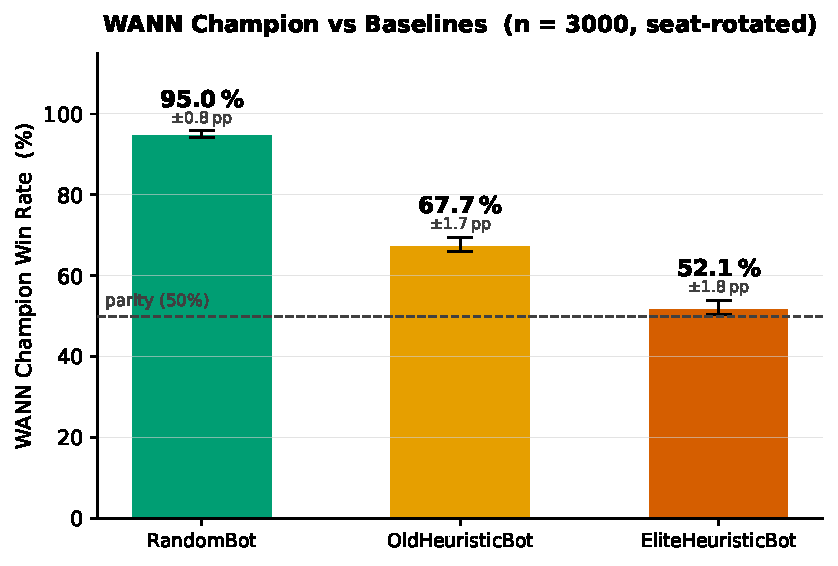
\includegraphics[width=0.72\textwidth,height=0.40\textheight,keepaspectratio]{../report/figures/tournament.pdf}
  \vspace{4pt}
  \begin{columns}[T]
    \column{0.48\textwidth}
      \centering
      \scriptsize
      \textbf{Tournament matrix} (win\%, $n=3000$)\\[2pt]
      \begin{tabular}{@{}lcccc@{}}
        \toprule
        & \scriptsize Rnd & \scriptsize Old & \scriptsize Elite & \scriptsize\textbf{WANN} \\
        \midrule
        Random   & 50.0 & 10.8 & 4.7  & 5.1 \\
        Old      & 89.2 & 50.0 & 32.5 & 32.3 \\
        Elite    & 95.3 & 67.5 & 50.0 & 47.9 \\
        \textbf{WANN} & \textbf{95.0} & \textbf{67.7} & \textbf{52.1} & 50.0 \\
        \bottomrule
      \end{tabular}
    \column{0.52\textwidth}
      \centering
      \begin{itemize}
        \item 95\% CI $[50.3\%, 53.9\%]$ \textbf{excludes 50\%}
        \item Card points: 60.2 vs.\ 59.8
        \item WANN vs.\ Old: 67.7\% (Elite: 67.5\%)
        \item Prior best \textbf{30.2\%}; first time the project beat Elite
      \end{itemize}
  \end{columns}
\end{frame}

% ======================================================================
% SLIDE 9 — The Journey (diagnosis-first approach)
% ======================================================================
\begin{frame}{Three root-cause fixes turned a collapsed network into an Elite-beating champion}
  \centering
  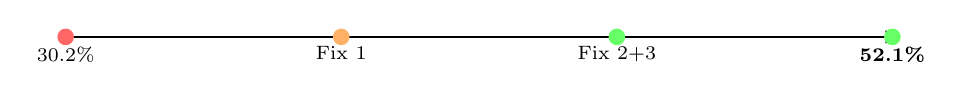
\begin{tikzpicture}
    \draw[->,thick] (0,0) -- (10.5,0) node[right] {};
    % Labels
    \node[below] at (0,0) {\scriptsize 30.2\%};
    \node[below] at (3.5,0) {\scriptsize Fix 1};
    \node[below] at (7.0,0) {\scriptsize Fix 2+3};
    \node[below] at (10.5,0) {\scriptsize\textbf{52.1\%}};
    % Markers
    \fill[red!60] (0,0) circle (3pt);
    \fill[orange!60] (3.5,0) circle (3pt);
    \fill[green!60] (7.0,0) circle (3pt);
    \fill[green!60] (10.5,0) circle (3pt);
  \end{tikzpicture}
  \vspace{8pt}
  \begin{columns}[T]
    \column{0.33\textwidth}
      \centering
      \textbf{Problem}\\[2pt]
      \scriptsize
      Network collapsed to\\``always EFFICIENT\_WIN''\\
      Intents unequally weak\\20\% / 37\% / 25\%
    \column{0.33\textwidth}
      \centering
      \textbf{Fix \#1}\\[2pt]
      \scriptsize
      \textbf{Styled resolver}\\
      Every intent $\approx$ Elite\\
      48\% / 47\% / 46\%\\
      Collapse $\rightarrow$ merely ties
    \column{0.33\textwidth}
      \centering
      \textbf{Fix \#2 \& \#3}\\[2pt]
      \scriptsize
      Best-of-3-intent labeling\\
      \textbf{Rollout teacher}\\
      62\% vs.\ Elite\\
      $\rightarrow$ 4.5$\times$ simpler
  \end{columns}
  \vspace{6pt}
  \centering
  \parbox{0.92\textwidth}{\centering\small\emph{Diagnosed with a training-free harness in seconds, not blind retraining in hours.}}
\end{frame}

% ======================================================================
% SLIDE 10 — Interpretability Payoff
% ======================================================================
\begin{frame}[fragile]{The follow brain compiles to 5 logic gates at depth 5 (verified behavior-preserving)}
  \centering
  \textbf{Compiled FOLLOW-brain rules} {\footnotesize(after constant-folding + alias inlining)}\\[6pt]
  \lstset{basicstyle=\footnotesize\ttfamily}
  \begin{lstlisting}[frame=single,backgroundcolor=\color{gray!5}]
hidden_42 = NOT(Holds_Boss_Led)
hidden_48 = (1 + Any_Opp_Void_Led)
hidden_41 = NOT((1 + h_42 + 2*hidden_48))
hidden_40 = THRESHOLD((h_41 + Trump_Count) > 0.5)
hidden_55 = THRESHOLD(hidden_40 > 0.5)
MAX_FORCE      = 2*Game_Pts_Remaining
EFFICIENT_WIN  = 0
EQUITY_BUILDER = 1 + 2*hidden_41 + hidden_55
\end{lstlisting}
  \vspace{6pt}
  \begin{columns}[T]
    \column{0.52\textwidth}
      \scriptsize
      \textbf{LEAD brain (10 gates, depth 6):}\\
      \texttt{EQUITY = THRESHOLD(NOT(Trump\_Count))}\\
      \texttt{MAX\_FORCE = (ahead \& point-dense}\\
      \texttt{\phantom{MAX\_FORCE = (}\& partner-winning)}\\
      \texttt{\phantom{MAX\_FORCE = }OR (no short side suit)}
    \column{0.48\textwidth}
      \scriptsize
      \textbf{EFFICIENT\_WIN $= 0$ in both brains:} the net never delegates to pure
      Elite; it always applies one of the two overlays.\\[4pt]
      \textit{Verified on 2000 random states: the removed symbols carry zero information.}
  \end{columns}
\end{frame}

% ======================================================================
% SLIDE 10b — Raw topology (full slide for legibility)
% ======================================================================
\begin{frame}{Before folding: the raw evolved follow-brain topology}
  \centering
  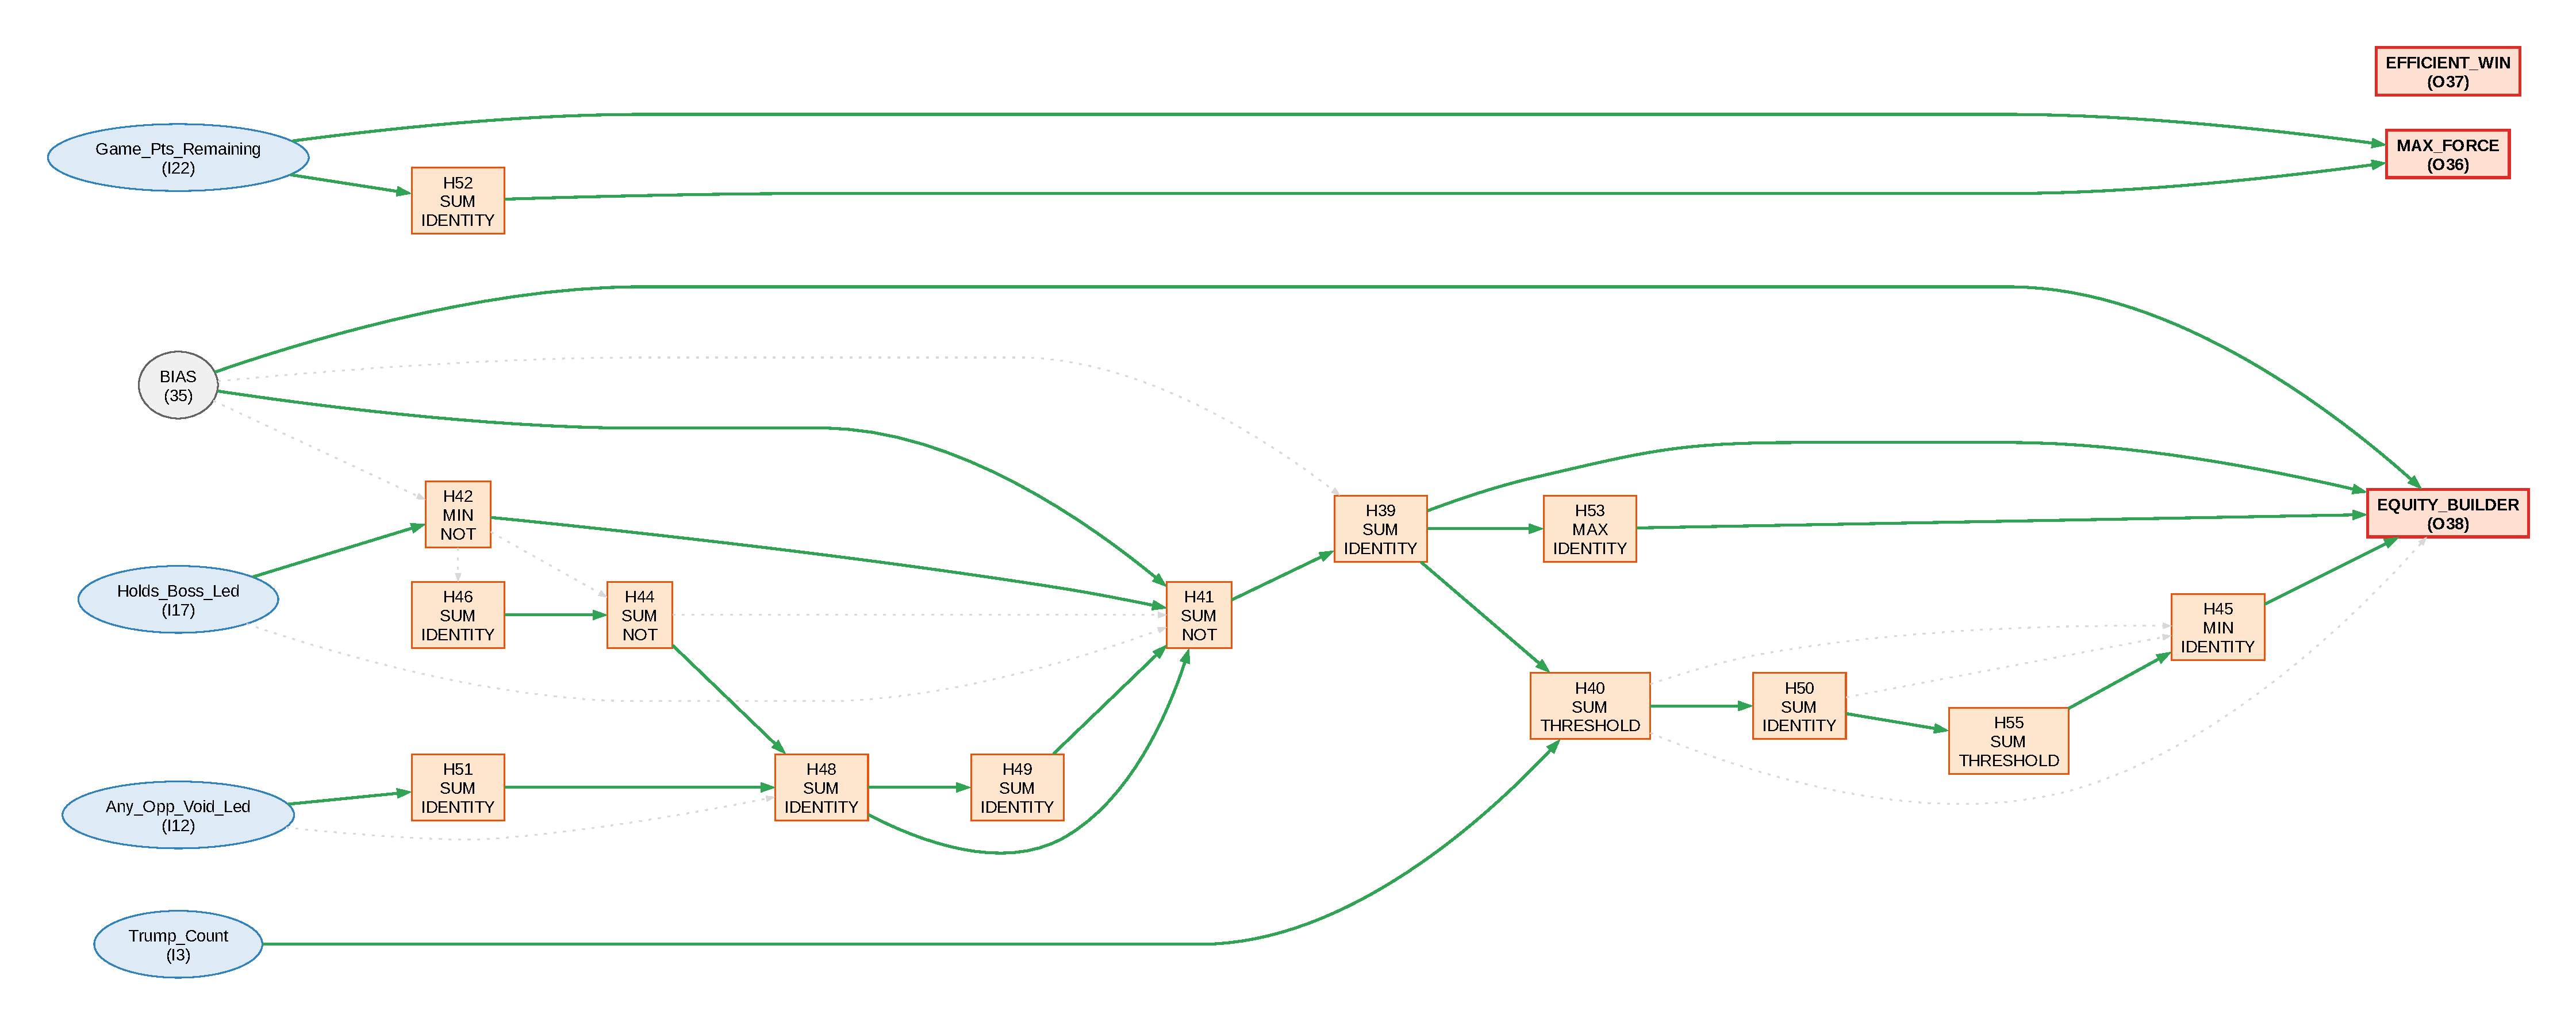
\includegraphics[width=\textwidth,height=0.80\textheight,keepaspectratio]{../report/figures/topology_follow.pdf}

  \vspace{2pt}
  {\scriptsize 17 hidden gates, 44 connections. Constant-folding and alias inlining collapse the
  \emph{active} logic to the \textbf{5 gates} on the previous slide, a 4.5$\times$ reduction
  versus the earlier champion.}
\end{frame}

% ======================================================================
% SLIDE 11 — Honest Analysis
% ======================================================================
\begin{frame}{The styled resolver that enabled the win also sets the strength ceiling, and we measured it}
  \centering
  \begin{tabular}{@{}lcccc@{}}
    \toprule
    & \textbf{Any pure intent} & \textbf{Final champion} & \textbf{3-intent oracle} & \textbf{RF ceiling} \\
    \midrule
    vs.\ Elite & 47--48\% & \textbf{52.1\%} & \textbf{58\%} & 63--71\% \\
    \bottomrule
  \end{tabular}
  \vspace{6pt}

  \footnotesize
  \textbf{Elite floor} \hspace{4pt} $\rightarrow$ \hspace{4pt}
  every intent $\approx$ Elite individually $\rightarrow$ collapse merely ties\\
  \textbf{Oracle cap} \hspace{4pt} $\rightarrow$ \hspace{4pt}
  perfect intent selection $\approx$ 58\% $\rightarrow$ $\sim$8 pp headroom left\\[4pt]
  \textbf{+2\% = the learned deviation overlay} on top of the fixed resolver base.

  \vspace{8pt}
  \begin{columns}[T]
    \column{0.50\textwidth}
      \footnotesize
      \textbf{What limits us}\\[4pt]
      \begin{itemize}
        \item 3 intents nearly equivalent in fitness
        \item Weak gradient for learned selection
        \item Lead decision harder: RF $+$2.5 pp
        \item Follow learnable: RF $+$7.9 pp
      \end{itemize}
    \column{0.50\textwidth}
      \footnotesize
      \textbf{What could raise the cap}\\[4pt]
      \begin{itemize}
        \item More-differentiated intents
        \item Opponent-card inference features
        \item Knowledge distillation
        \item Richer belief state
      \end{itemize}
  \end{columns}
  \vspace{2pt}
  \centering
  \parbox{0.92\textwidth}{\centering\footnotesize\emph{We measure and report our ceiling; $+2\%$ is the learned overlay.}}
\end{frame}

% ======================================================================
% SLIDE 12 — Live Demo / Website
% ======================================================================
\begin{frame}{You can explore the champion's decision-making interactively in the browser}
  \centering
  \vspace{4pt}
  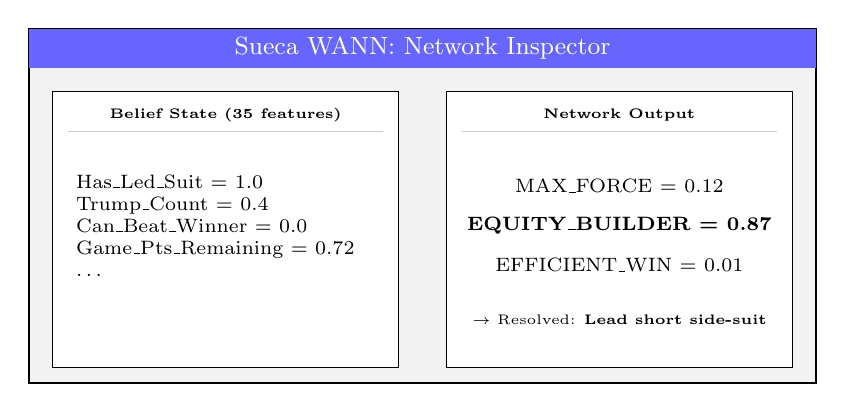
\begin{tikzpicture}
    % Browser window mockup
    \fill[black!5] (0,0) rectangle (10,4.5);
    \draw[thick] (0,0) rectangle (10,4.5);
    % Title bar
    \fill[blue!60] (0,4.0) rectangle (10,4.5);
    \node[white] at (5,4.25) {\small Sueca WANN: Network Inspector};
    % Content boxes
    \fill[white] (0.3,0.2) rectangle (4.7,3.7);
    \draw (0.3,0.2) rectangle (4.7,3.7);
    \node[font=\tiny] at (2.5,3.4) {\textbf{Belief State (35 features)}};
    \draw[gray!40] (0.5,3.2) -- (4.5,3.2);
    \node[font=\scriptsize,text width=3.8cm,align=left] at (2.5,2.0)
      {Has\_Led\_Suit = 1.0\\Trump\_Count = 0.4\\Can\_Beat\_Winner = 0.0\\Game\_Pts\_Remaining = 0.72\\\ldots};
    \fill[white] (5.3,0.2) rectangle (9.7,3.7);
    \draw (5.3,0.2) rectangle (9.7,3.7);
    \node[font=\tiny] at (7.5,3.4) {\textbf{Network Output}};
    \draw[gray!40] (5.5,3.2) -- (9.5,3.2);
    \node[font=\scriptsize] at (7.5,2.5) {MAX\_FORCE = 0.12};
    \node[font=\scriptsize] at (7.5,2.0) {\textbf{EQUITY\_BUILDER = 0.87}};
    \node[font=\scriptsize] at (7.5,1.5) {EFFICIENT\_WIN = 0.01};
    \node[font=\tiny] at (7.5,0.8) {$\rightarrow$ Resolved: \textbf{Lead short side-suit}};
  \end{tikzpicture}
  \vspace{4pt}
  \begin{center}
    \small\textbf{React + WASM}: Rust game engine compiled to WebAssembly\\
    Play Sueca against the WANN, watch the logic flow in real time.
  \end{center}
\end{frame}

% ======================================================================
% SLIDE 13 — Future Work & Conclusion
% ======================================================================
\begin{frame}{Richer intents and opponent-card inference are the path to breaking the 58\% ceiling}
  \begin{columns}[T]
    \column{0.52\textwidth}
      \footnotesize
      \textbf{Future directions}\\[4pt]
      \begin{enumerate}
        \item \textbf{Richer intents}\\
              more-differentiated play styles\\
              $\rightarrow$ raise the oracle cap above 58\%
        \item \textbf{Opponent-card inference}\\
              can a logic circuit learn to infer\\
              hidden cards from optimal play?
        \item \textbf{Knowledge distillation}\\
              champion $\rightarrow$ even smaller student\\
              $\rightarrow$ Pareto curve of strength vs.\ size
      \end{enumerate}
    \column{0.48\textwidth}
      \footnotesize
      \textbf{What we showed}\\[4pt]
      \begin{itemize}
        \item Evolved an \textbf{interpretable},\\Elite-beating Sueca agent
        \item Verified pipeline:\\
              logic gates $\rightarrow$ \textbf{5 readable rules}
        \item Honest analysis of the\\resolver-floor ceiling
        \item Supra-Elite rollout teacher\\
              ($\sim$1000$\times$ cheaper)
        \item All code, data, and rules\\are reproducible
      \end{itemize}
  \end{columns}
  \vspace{4pt}
  \centering
  \textbf{Competitive, interpretable card-play AI is possible: the rules fit on one slide.}
\end{frame}

% ======================================================================
% SLIDE 14 — Q&A / Backup
% ======================================================================
\begin{frame}{Thank you. Questions?}
  \centering
  \vspace{8pt}
  \textbf{Key references}\\[4pt]
  \begin{tabular}{@{}ll@{}}
    \toprule
    Gaier \& Ha 2019 & Weight-Agnostic Neural Networks\\
    Stanley \& Miikkulainen 2002 & NEAT\\
    Mouret \& Clune 2015 & MAP-Elites\\
    Reisinger et al.\ 2004 & Coevolving modular (L-NEAT)\\
    \bottomrule
  \end{tabular}
  \vspace{12pt}
  \textbf{Reproducibility}\\[4pt]
  \scriptsize
  All commands in \texttt{README.md}\\
  Canonical champion: \texttt{checkpoints/production/2026-06-14-2/}\\
  \texttt{cargo build -p sueca\_wann --release \&\& cargo test --all}
  \vspace{10pt}
  \begin{center}
    \normalsize André Cardoso\\
    \small DETI, Universidade de Aveiro
  \end{center}
\end{frame}

\end{document}
